\documentclass[cal1spr16Lectures.tex]{subfiles}

\begin{document}

%\section[Week 9]{Week 9: 14-18 Mar}

% % % 
\subsubsection{\bf Monday 14 March}
% % %

\begin{frame}[allowframebreaks]{$\pi$ Day 2016}
\begin{itemize}\footnotesize
\item Exam 2: Curve, etc. is posted. 

\begin{center}
\includegraphics[scale=0.6]{..//Exam2Spread}
\end{center}
\framebreak
\item Midterm: expect it back Thursday in drill.  Don't expect a curve. :(
\item ``Fast Track Calculus": Dr. Kathleen Morris will be teaching a second 8 weeks Calculus One class.  ``If you have a student who is maybe doing poorly because of illness or a tragic event in their life during the beginning of the semester, this might be an opportunity for a new start for them."  The class requires departmental consent so the student will need to contact Kathleen to get permission to enroll.
\end{itemize}
\end{frame}

% % %
\subsubsection{Steps for Solving Related Rates Problems}
% % % 

% % %
\begin{frame}{\small Steps for Solving Related Rates Problems}
\small
\begin{itemize}
\item[1.] Read the problem carefully, making a sketch to organize the given information.  Identify the rates that are given and the rate that is to be determined.
\item[2.] Write one or more equations that express the basic relationships among the variables.
\item[3.] Introduce rates of change by differentiating the appropriate equation(s) with respect to time $t$.
\item[4.] Substitute known values and solve for the desired quantity.
\item[5.] Check that the units are consistent and the answer is reasonable.
\end{itemize}
\end{frame}

% % %
\begin{frame}
\frametitle{}
\begin{block}{The Jet Problem}
A jet ascends at a $10^{\circ}$ angle from the horizontal with an airspeed of 550 miles/hr (its speed along its line of flight is 550 miles/hr).  How fast is the altitude of the jet increasing?  If the sun is directly overhead, how fast is the shadow of the jet moving on the ground?
\end{block}
\end{frame}

% % %
\begin{frame}
\small
{\bf Step 1:}  There are three variables:  the distance the shadow has traveled ($x$), the altitude of the jet ($h$), and the distance the jet has actually traveled on its line of flight ($z$).  We know that $\textstyle\frac{dz}{dt}=550\ \text{miles/hr}$ and we want to find $\textstyle\frac{dx}{dt}$ and $\textstyle\frac{dh}{dt}$.  We also see that these variables are related through a right triangle:
\begin{center}
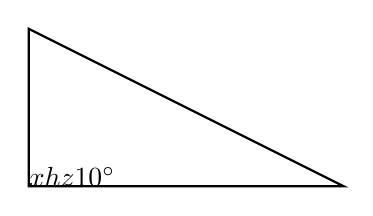
\begin{tikzpicture}[thick]
\coordinate (O) at (0,0);
\coordinate (A) at (4,0);
\coordinate (B) at (0,2);
\draw (O)--(A)--(B)--cycle;
\tkzLabelSegment[below=2pt](O,A){$x$}
\tkzLabelSegment[left=2pt](O,B){$h$}
\tkzLabelSegment[above right=2pt](A,B){$z$}
%\tkzMarkAngle[fill= orange,size=0.65cm,opacity=.4](A,O,B)
%\tkzLabelAngle[pos = 0.35](A,O,B){$\gamma$}
\tkzMarkAngle[size=0.7cm,opacity=.4](B,A,O)
\tkzLabelAngle[pos = 1.3](B,A,O){$10^{\circ}$}
%\tkzMarkAngle[fill= orange,size=0.7cm,opacity=.4](O,B,A)
%\tkzLabelAngle[pos = 0.5](O,B,A){$\beta$}
\end{tikzpicture}
\end{center}
\end{frame}

% % %
\begin{frame}
\small
{\bf Step 2:}  To answer how fast the altitude is increasing, we need an equation involving only $h$ and $z$.  Using trigonometry,
\[\sin(10^{\circ})=\frac{h}{z} \implies h=\sin(10^{\circ}) \cdot z.\]

\vspace{1pc}
To answer how fast the shadow is moving, we need an equation involving only $x$ and $z$.  Using trigonometry,
\[\cos(10^{\circ})=\frac{x}{z} \implies x=\cos(10^{\circ}) \cdot z.\]
\end{frame}

% % %
\begin{frame}
\footnotesize
{\bf Step 3:}  We can now differentiate each equation to answer each question:
\begin{alignat*}{2}
h=\sin(10^{\circ}) \cdot z &\implies \dfrac{dh}{dt}=\sin(10^{\circ}) \dfrac{dz}{dt} \\
x=\cos(10^{\circ}) \cdot z &\implies \dfrac{dx}{dt}=\cos(10^{\circ}) \dfrac{dz}{dt}
\end{alignat*}

\vspace{1pc}
{\bf Step 4:}  We know that $\textstyle\frac{dz}{dt}=550\ \text{miles/hr}$.  So 
\begin{alignat*}{2}
\dfrac{dh}{dt} &=\sin(10^{\circ}) \cdot 550 \approx 95.5\ \text{miles/hr}\\
\dfrac{dx}{dt} &=\cos(10^{\circ}) \cdot 550 \approx 541.6\ \text{miles/hr}
\end{alignat*}
\end{frame}

% % %
\begin{frame}
\frametitle{}
{\bf Step 5:}  Because both answers are in terms of miles/hr and both answers seem reasonable within the context of the problem, we conclude that the jet is gaining altitude at a rate of 95.5 miles/hr, while the shadow on the ground is moving at about 541.6 miles/hr.
\end{frame}

% % %
\begin{frame}\small
\begin{ex} The sides of a cube increase at a rate of $R$ cm/sec.  When the sides have a length of 2 cm, what is the rate of change of the volume? \end{ex}
%
%\begin{ex} Two boats leave a dock at the same time.  One boat travels south at 30 miles/hr and the other travels east at 40 miles/hr.  After half an hour, how fast is the distance between the boats increasing? \end{ex}
\end{frame}

% % %
\begin{frame}
\begin{exe}
A 13 foot ladder is leaning against a vertical wall when Jack begins pulling the foot of the ladder away from the wall at a rate of 0.5 ft/sec.  How fast is the top of the ladder sliding down the wall when the foot of the ladder is 5 ft from the wall?
\end{exe}
\end{frame}

% % %
\begin{frame}
\begin{exe}
Sand falls from an overhead bin and accumulates in a conical pile with a radius that is always three times its height.  Suppose the height of the pile increases at a rate of 2 cm/sec.  When the pile is 12 cm high, at what rate is the sand leaving the bin?  \emph{Recall the volume of a cone: $V=\textstyle\frac{1}{3}\pi r^2h$.}
\end{exe}
\end{frame}

% % % 
\subsubsection{Book Problems}
% % % 

% % %
\begin{frame}
\begin{block}{3.11 Book Problems}
5-14, 16-19, 21-24, 37-38
\end{block}
\end{frame}

\end{document}